\documentclass{article}

\usepackage{graphicx}
\usepackage{tikz}
\usepackage{tikzsymbols}
\usetikzlibrary{calc,patterns,shapes.geometric}
\pagestyle{empty}
\usepackage[margin=0pt]{geometry}
\geometry{papersize={14in,12in}}

\def\centerarc[#1](#2)(#3:#4:#5){\draw[#1] ($(#2)+({#5*cos(#3)},{#5*sin(#3)})$) arc (#3:#4:#5);}

\begin{document}
	\begin{figure}
		\centering
		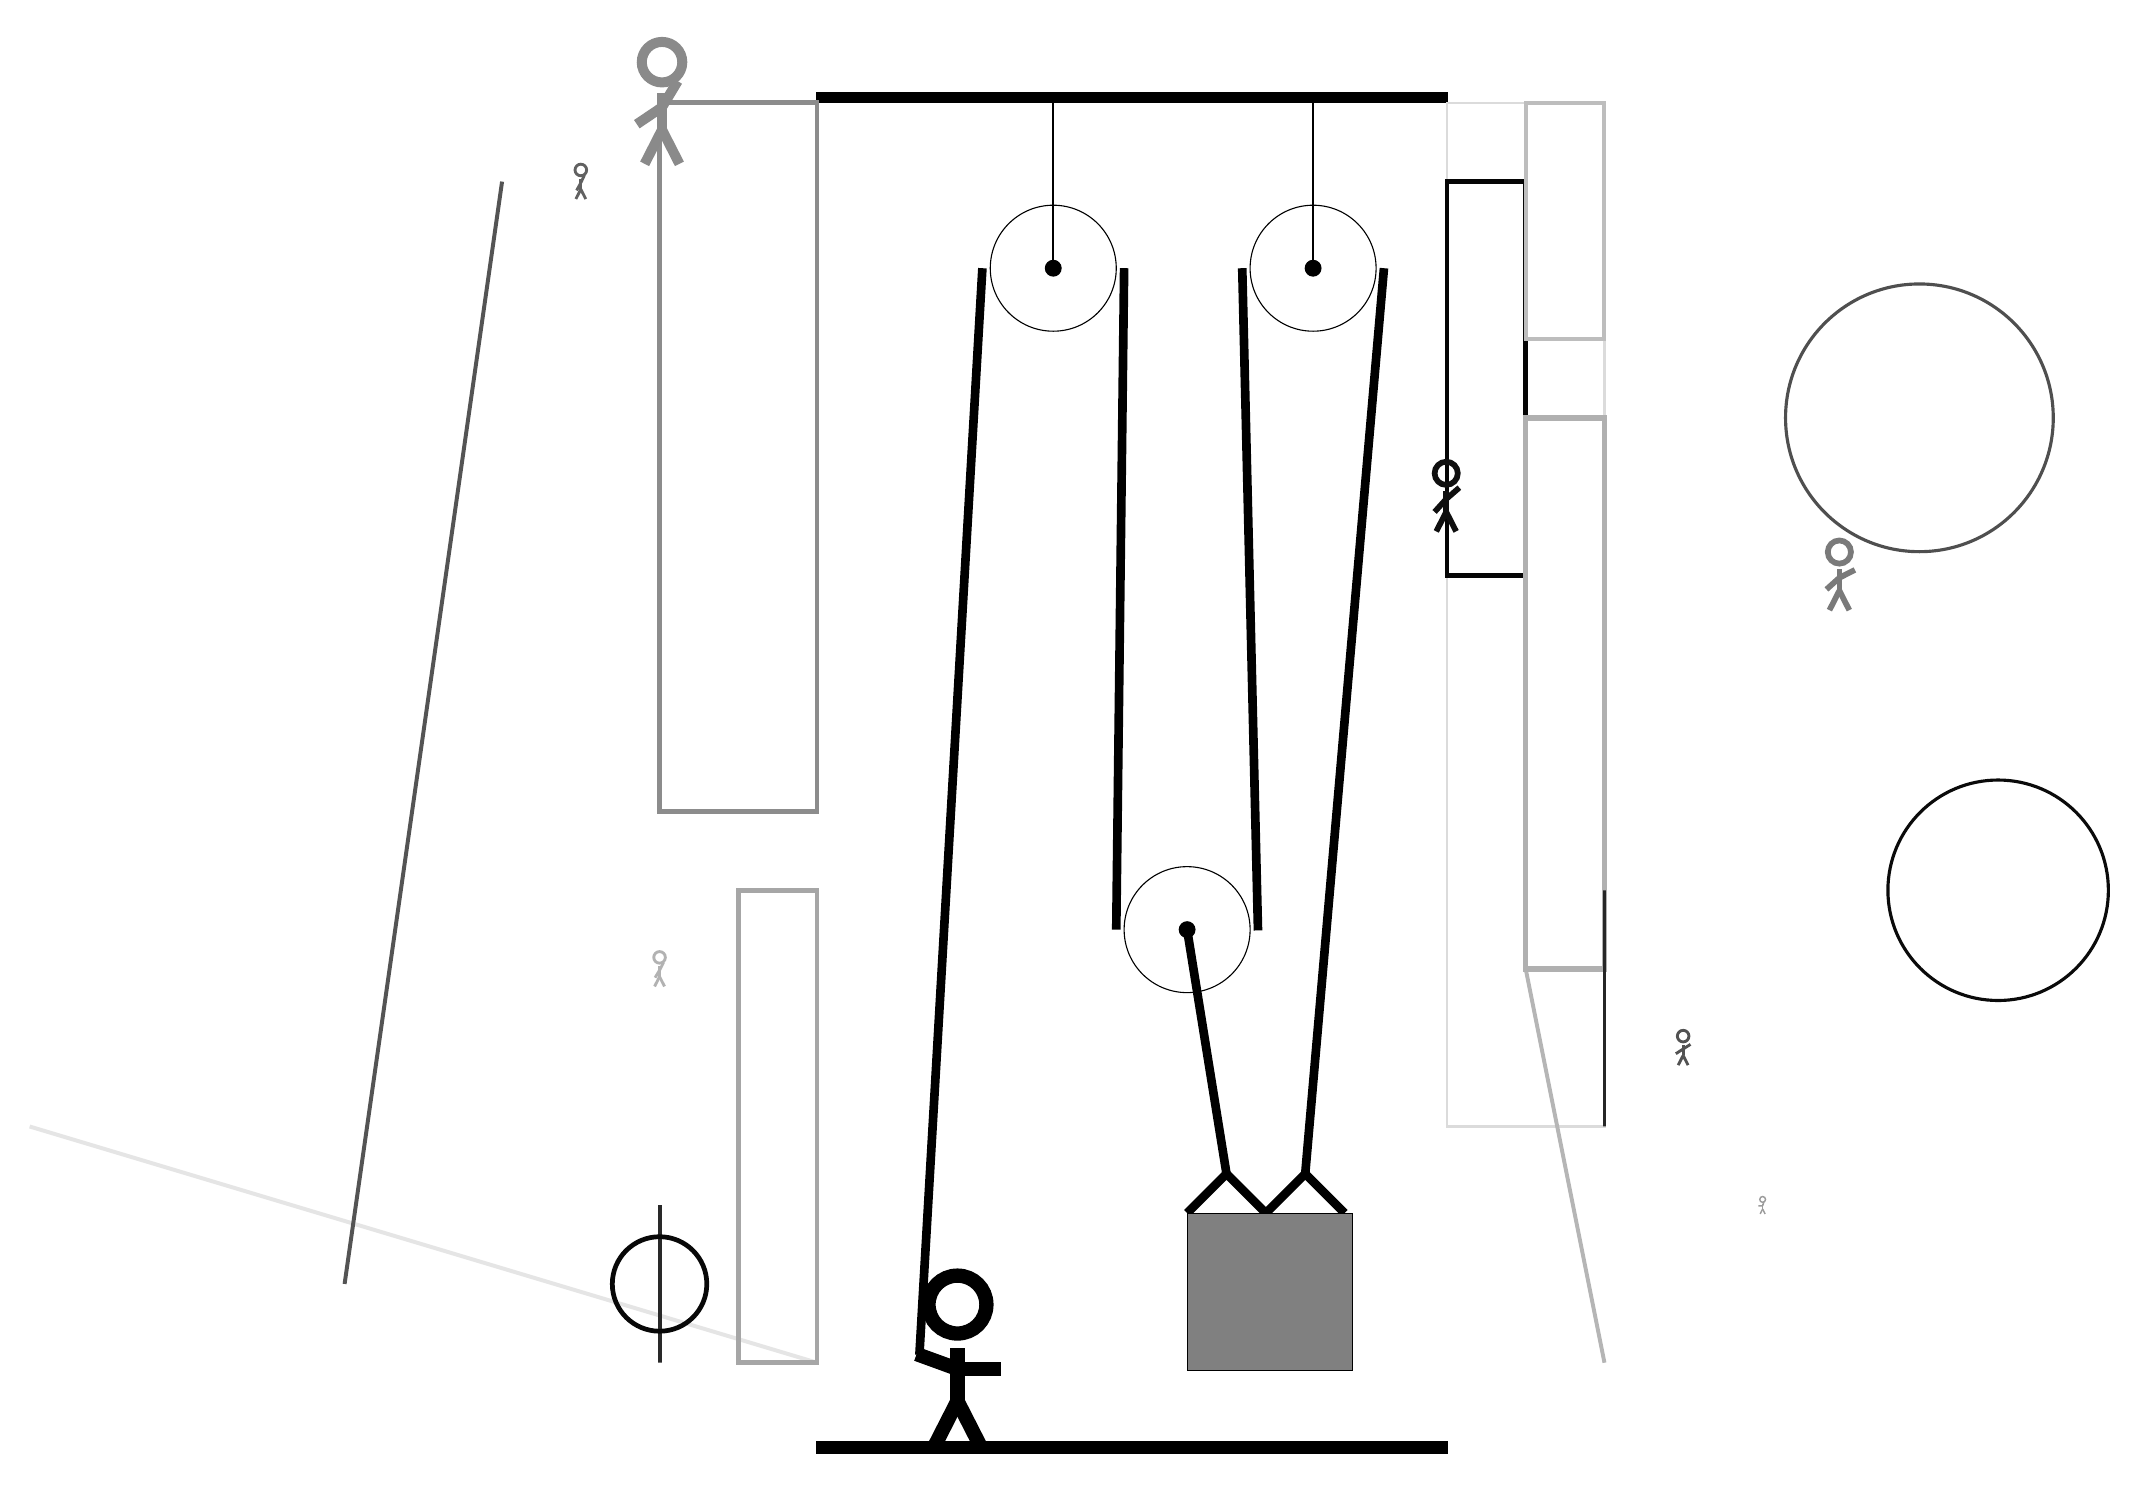
\begin{tikzpicture}
			%%%%% START %%%%%
			
			\draw[fill=black] (-2, 14) rectangle (6, 14.125);
			
			\node[line width=0.2mm, color=black!68] at (9, 2) {\Strichmaxerl[2][33][32]};
			
			\draw[line width=0.3mm, color=black!14] (8, 1) rectangle (6, 14);
			\node[line width=0.6mm, color=black!39] at (10, 0) {\Strichmaxerl[1][1][72]};
			\draw[line width=0.6mm, color=black!98] (7, 13) rectangle (6, 8);
			\draw[line width=0.5mm, color=black!26] (7, 14) rectangle (8, 11);
			\draw[line width=0.5mm, color=black!10](-2, -2) -- (-12, 1);
			
			\draw [line width=0.4mm, color=black!96](13, 4) circle (1.4);
			\node[line width=0.5mm, color=black!94] at (6, 9) {\Strichmaxerl[4][48][41]};
			\draw[line width=0.5mm, color=black!84] (-4, -2) rectangle (-4, 0);
			\node[line width=0.5mm, color=black!30] at (-4, 3) {\Strichmaxerl[2][59][63]};
			\draw [line width=0.4mm, color=black!69](12, 10) circle (1.7);
			
			\draw[line width=0.5mm, color=black!29](7, 3) -- (8, -2);
			\node[line width=0.3mm, color=black!62] at (-5, 13) {\Strichmaxerl[2][61][65]};
			
			\draw[line width=0.6mm, color=black!35] (-2, -2) rectangle (-3, 4);
			\draw[line width=0.6mm, color=black!45] (-4, 14) rectangle (-2, 5);
			\node[line width=0.2mm, color=black!52] at (11, 8) {\Strichmaxerl[4][42][27]};
			
			\draw[line width=0.7mm, color=black!31] (7, 10) rectangle (8, 3);
			\node[line width=0.4mm, color=black!46] at (-4, 14) {\Strichmaxerl[7][34][59]};
			\draw[line width=0.3mm, color=black!85] (8, 1) rectangle (8, 4);
			\draw [line width=0.6mm, color=black!97](-4, -1) circle (0.6);
			\draw[line width=0.5mm, color=black!67](-6, 13) -- (-8, -1);
			
			
			\draw (1, 11.9) circle (0.8);
			\draw[fill=black] (1, 11.9) circle (0.1);
			\draw[thick] (1, 11.9) -- (1, 14);
			
			\draw (4.3, 11.9) circle (0.8);
			\draw[fill=black] (4.3, 11.9) circle (0.1);
			\draw[thick] (4.3, 11.9) -- (4.3, 14);
			
			\draw (2.7, 3.5) circle (0.8);
			\draw[fill=black] (2.7, 3.5) circle (0.1);
			
			\draw[line width=1.1mm]  (2.7, -0.1) -- (3.2, 0.4) -- (3.7, -0.1) -- (4.2, 0.4) -- (4.7, -0.1);
			\draw[fill=black!50] (2.7, -0.1) rectangle (4.8, -2.1);
			
			\draw[line width=1.1mm](-0.7, -1.9) -- (0.1, 11.9);
			\centerarc[line width=1.1mm](1, 11.9)(0:180:0.9);
			\draw[line width=1.1mm](1.9, 11.9) -- (1.8, 3.5);
			\centerarc[line width=1.1mm](2.7, 3.5)(180:370:0.9);
			\draw[line width=1.1mm] (3.6, 3.49) -- (3.4, 11.9);
			\centerarc[line width=1.1mm](4.3, 11.9)(0:180:0.9);
			\draw[line width=1.1mm](4.2, 0.4) -- (5.2, 11.9);
			\draw[line width=1.1mm] (3.2, 0.4) -- (2.7, 3.5);
			
			\node at (-0.2, -2) {\Strichmaxerl[10][-20][0]};
			
			\draw[fill=black] (-2, -3) rectangle (6, -3.15);
			
			%%%%% END %%%%%
		\end{tikzpicture}
	\end{figure}	
\end{document}